\documentclass[a4paper,12pt]{article}
\usepackage{blindtext}
\usepackage[utf8]{inputenc}
\usepackage{graphicx}
\usepackage{enumitem}
\usepackage{booktabs}
\usepackage{verbatim}
\usepackage{makecell}

\begin{document}
\begin{titlepage}
\center

\textsc{\LARGE User Manual}\\[1.5cm]
\textsc{\Large Project: Traffic Camera Image Analysis}\\[1.5cm]
\textsc{\large Client: DPSS, CSIR}\\[0.5cm]
\textsc{\large Team: Quadcore Productions}\\[0.5cm]

\begin{minipage}{0.4\textwidth}
\begin{flushleft} \large
\textbf{Author(s):}\\
Mpho \textsc{Baloyi}\\
Hlengekile \textsc{Jita}\\
Mayimela \textsc{Moses}\\
Mbhele \textsc{Themba}\\
\end{flushleft}
\end{minipage}
~
\begin{minipage}{0.4\textwidth}
\begin{flushright} \large
\textbf{Student number(s):} \\
14133670\\ % Student number
14077893\\
14019702\\
14007950\\
\end{flushright}
\end{minipage}\\


\includegraphics[width=\textwidth]{2012-quad-core-phones.jpg}

{\large University of Pretoria, Department of Computer Science}\\

{\large 23 October 2016}\\[3cm]

\vfil

\end{titlepage}

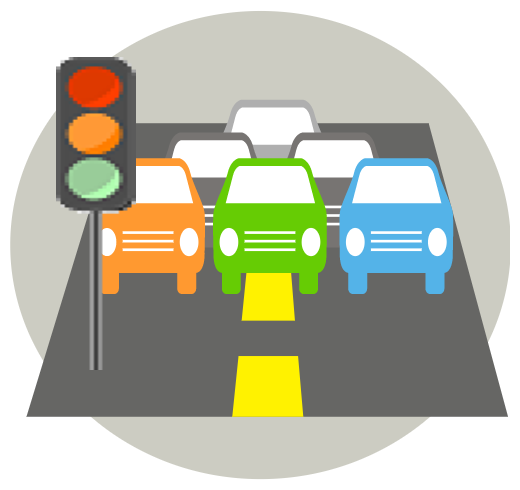
\includegraphics[width=\textwidth]{images/coverPage.png}
\begin{center}
\textsc{\textbf{\LARGE Traffic 411}}\\[1.5cm]
\textsc{\Large Android Application User Manual}\\[0.5cm]
\end{center}

\newpage
\tableofcontents
\newpage

\newpage
%\begin{comment}
\begin{table}[ht]
 \centering
 \caption{Version History}
 \label{tab:table1}
 \begin{tabular}{cccc}
   \toprule
    Version No. & Date & Changes & By\\
    \midrule
    1 & 29 July 2016 & \makecell{Application Installation, \\ Application Use} & \makecell{Mpho Baloyi,\\ Hlengekile Jita,\\ Moses Mayimela,\\ Themba Mbhele} \\
   2 & 23 October 2016 & \makecell{Added Screenshots \\ Updated Application Use} & \makecell{Mpho Baloyi,\\ Hlengekile Jita,\\ Moses Mayimela,\\ Themba Mbhele} \\
    \bottomrule
  \end{tabular}
\end{table}
%\end{comment}
\newpage

\section{Application Installation}
In order to install this application you will need the following:
\begin{itemize}
\item An Android Device
\item The Traffic 411 APK file
\end{itemize}

The Traffic 411 apk can be installed as follows:
\begin{enumerate}
\item \textbf{Make sure that third party apps are allowed on your device -} Go to Menu, then go to Settings, then go to Security and check the Unknown Sources option. This allow allow applications which aren't from the play store to be installed.
\item \textbf{Place the APK file in your device} 
\item \textbf{Install the application -} Select the APK file and it will install on your device
\end{enumerate}

Open up the application by selecting it in your Apps window. Once opened you will get the following screen, simply touch the logo to get started.
<<<<<<< HEAD
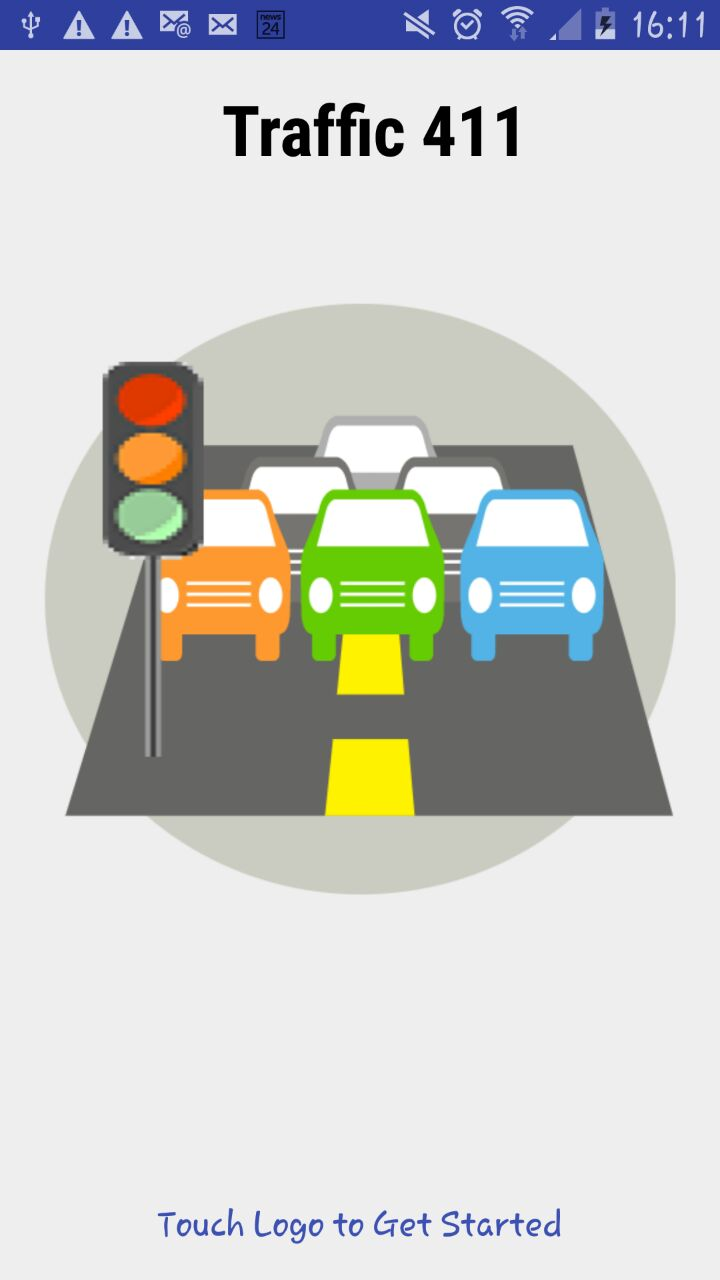
\includegraphics[width=\textwidth]{images/splashScreen.jpg}
=======
\begin{center}
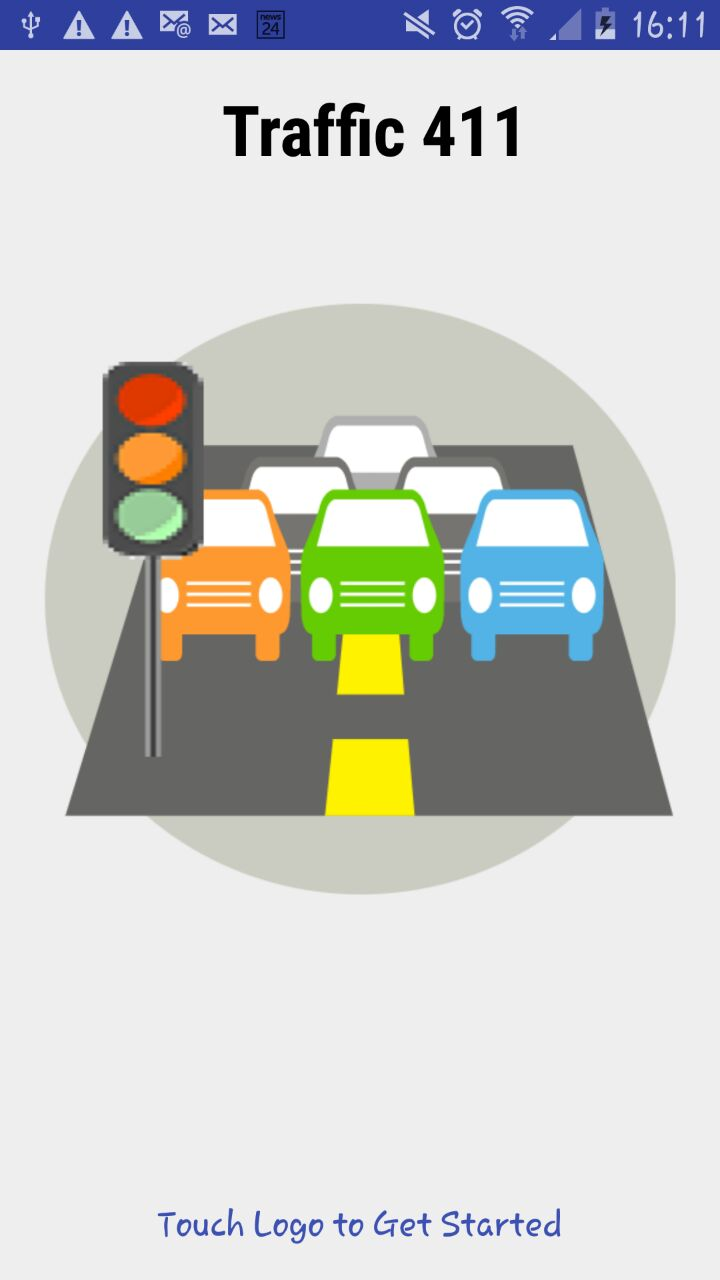
\includegraphics[width=50mm]{images/splashScreen.png}
\end{center}
>>>>>>> 4fb914f7de7a370f4cfd1de83509887d9d6942a3

\section{Application Use}
\subsubsection{Adding a Route}
The process of adding a route is as follows:
\begin{center}
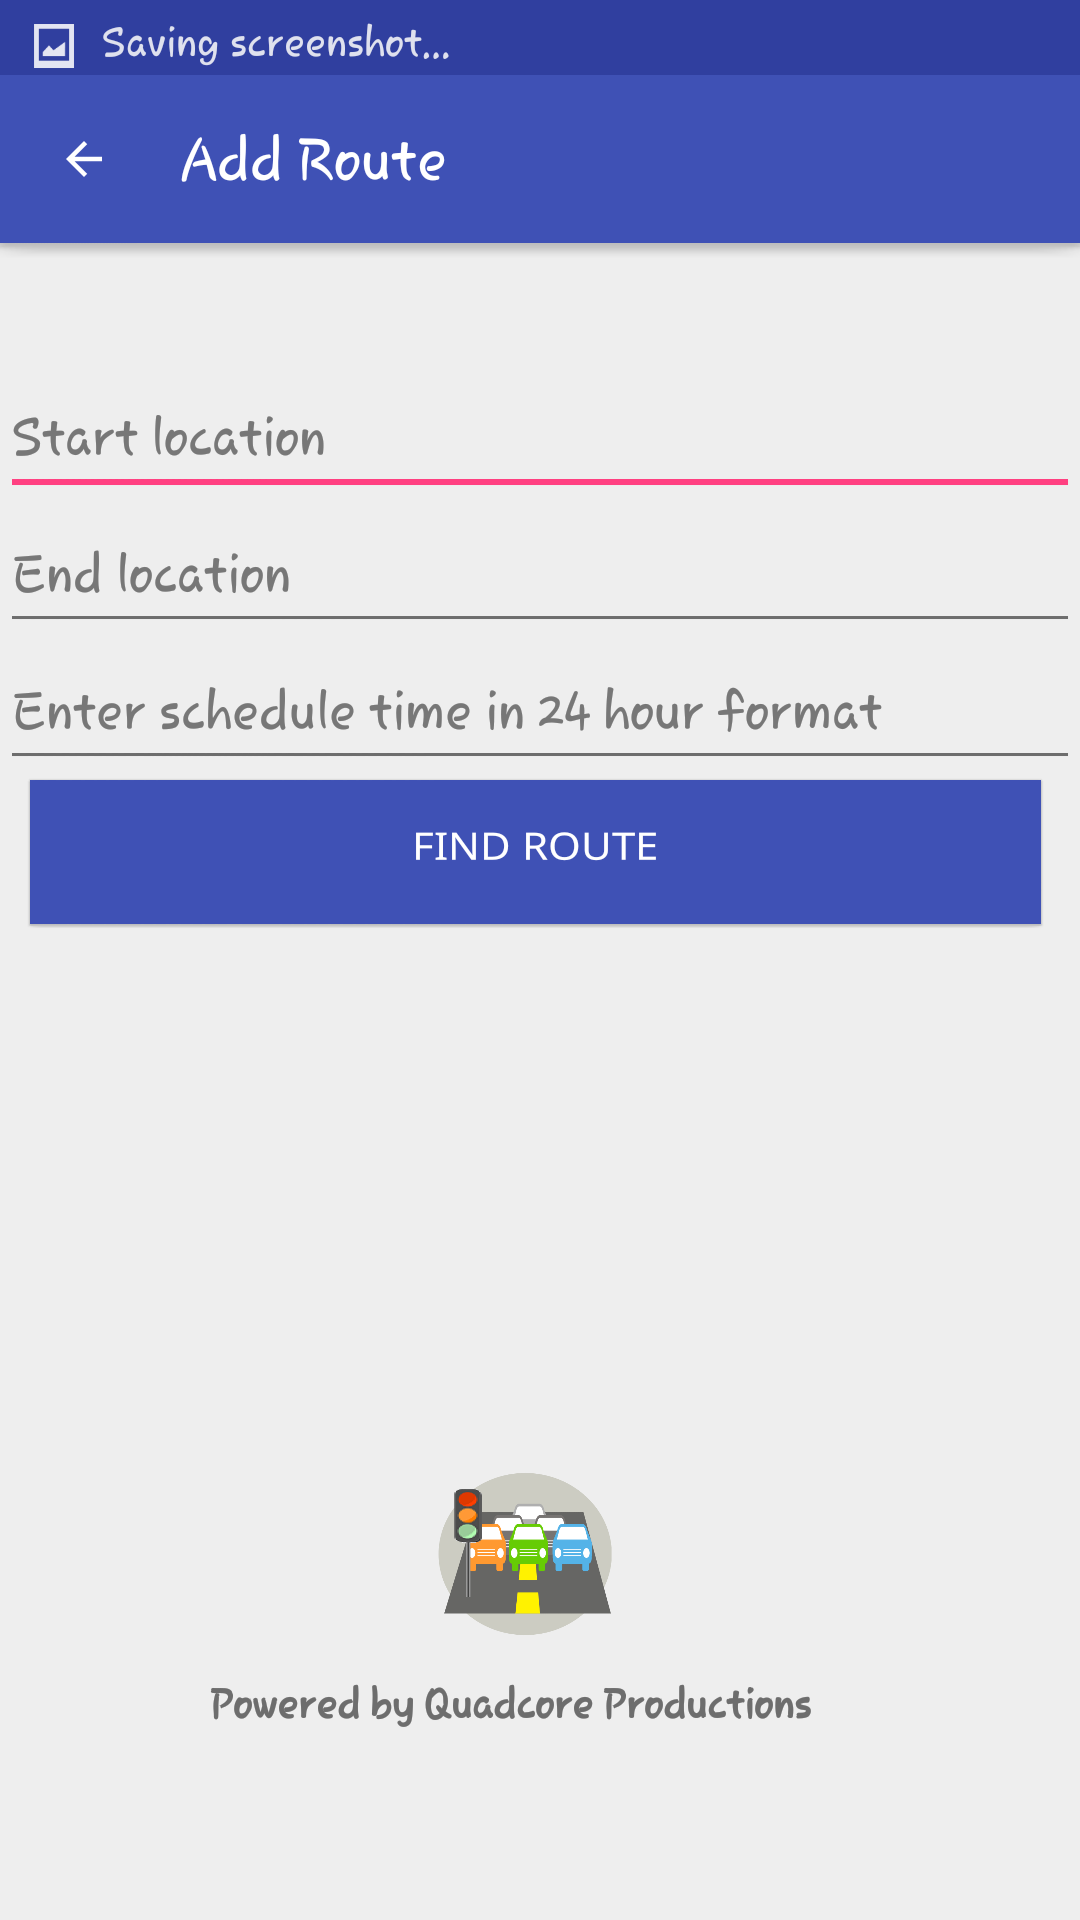
\includegraphics[width=50mm, scale=0.5]{images/AddRoute.png}
\end{center}
\begin{center}
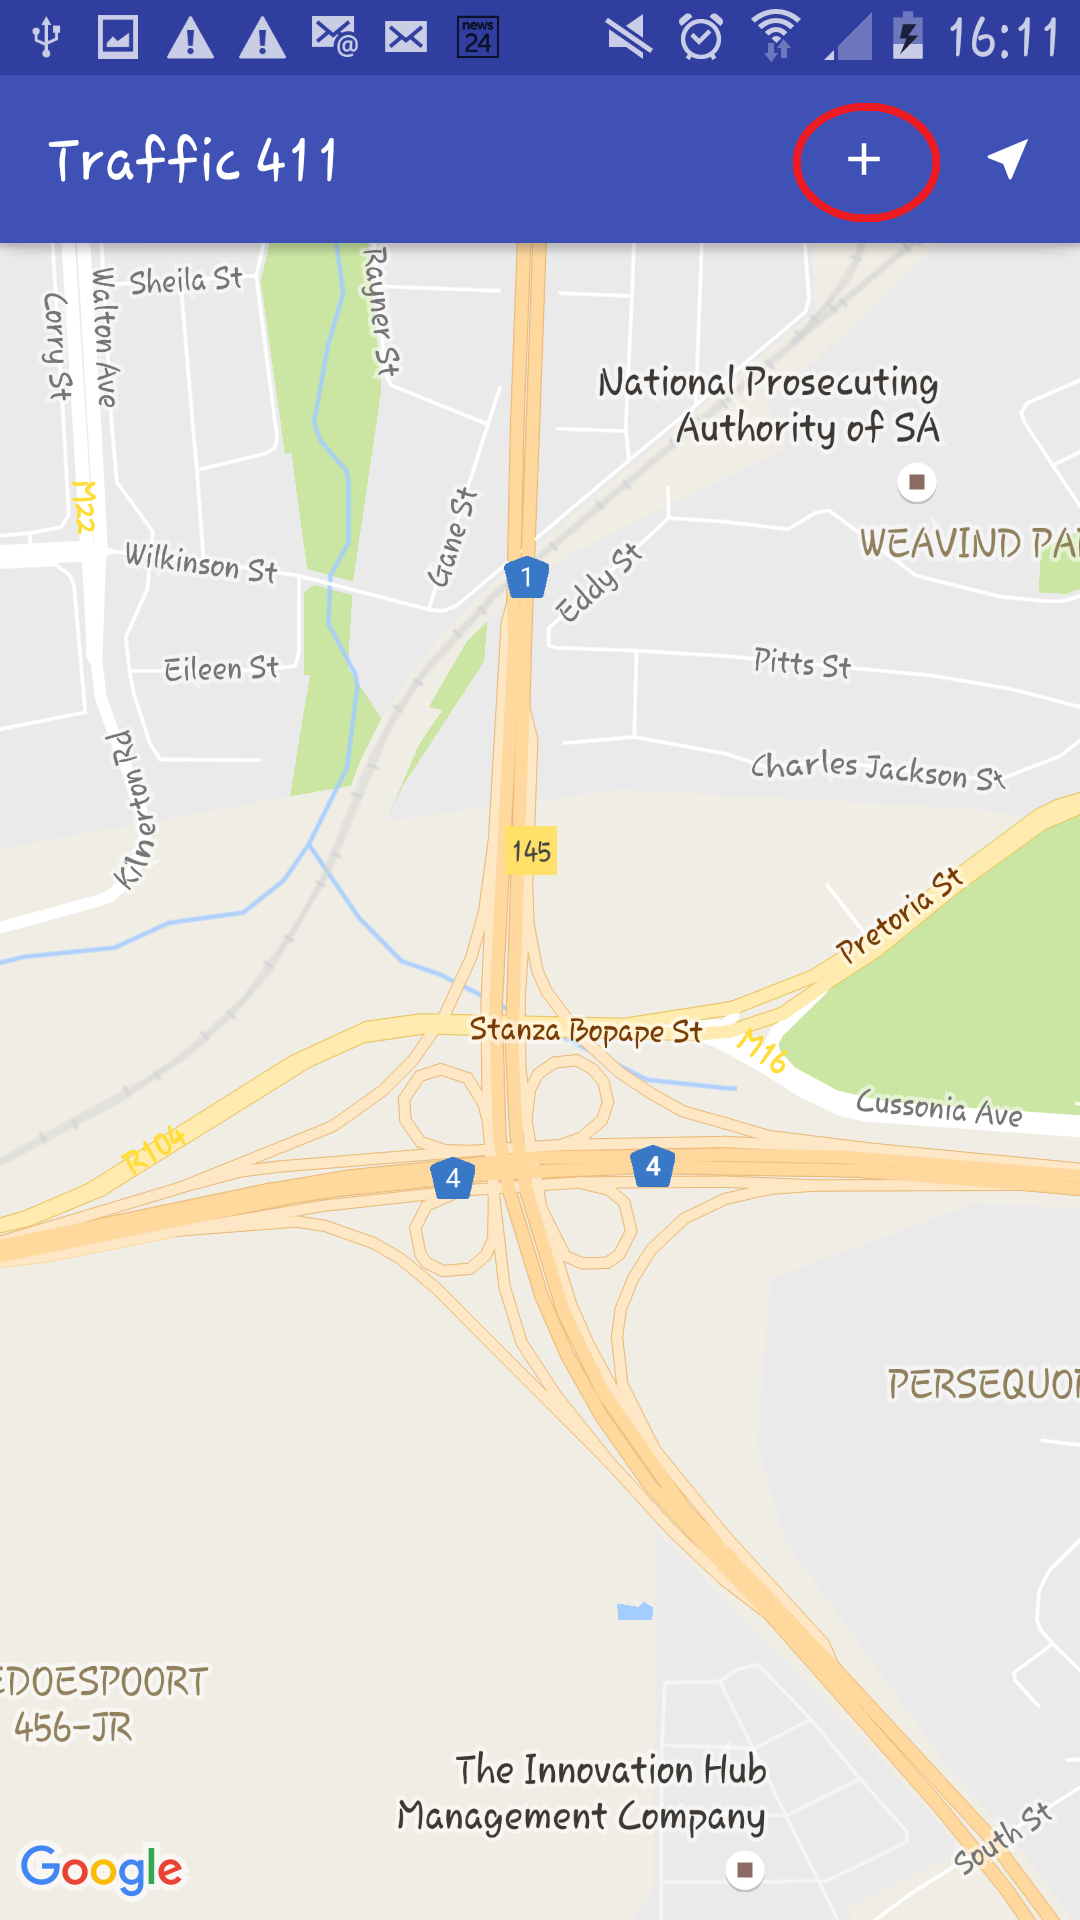
\includegraphics[width=50mm, scale=0.5]{images/MainScreen2.png}
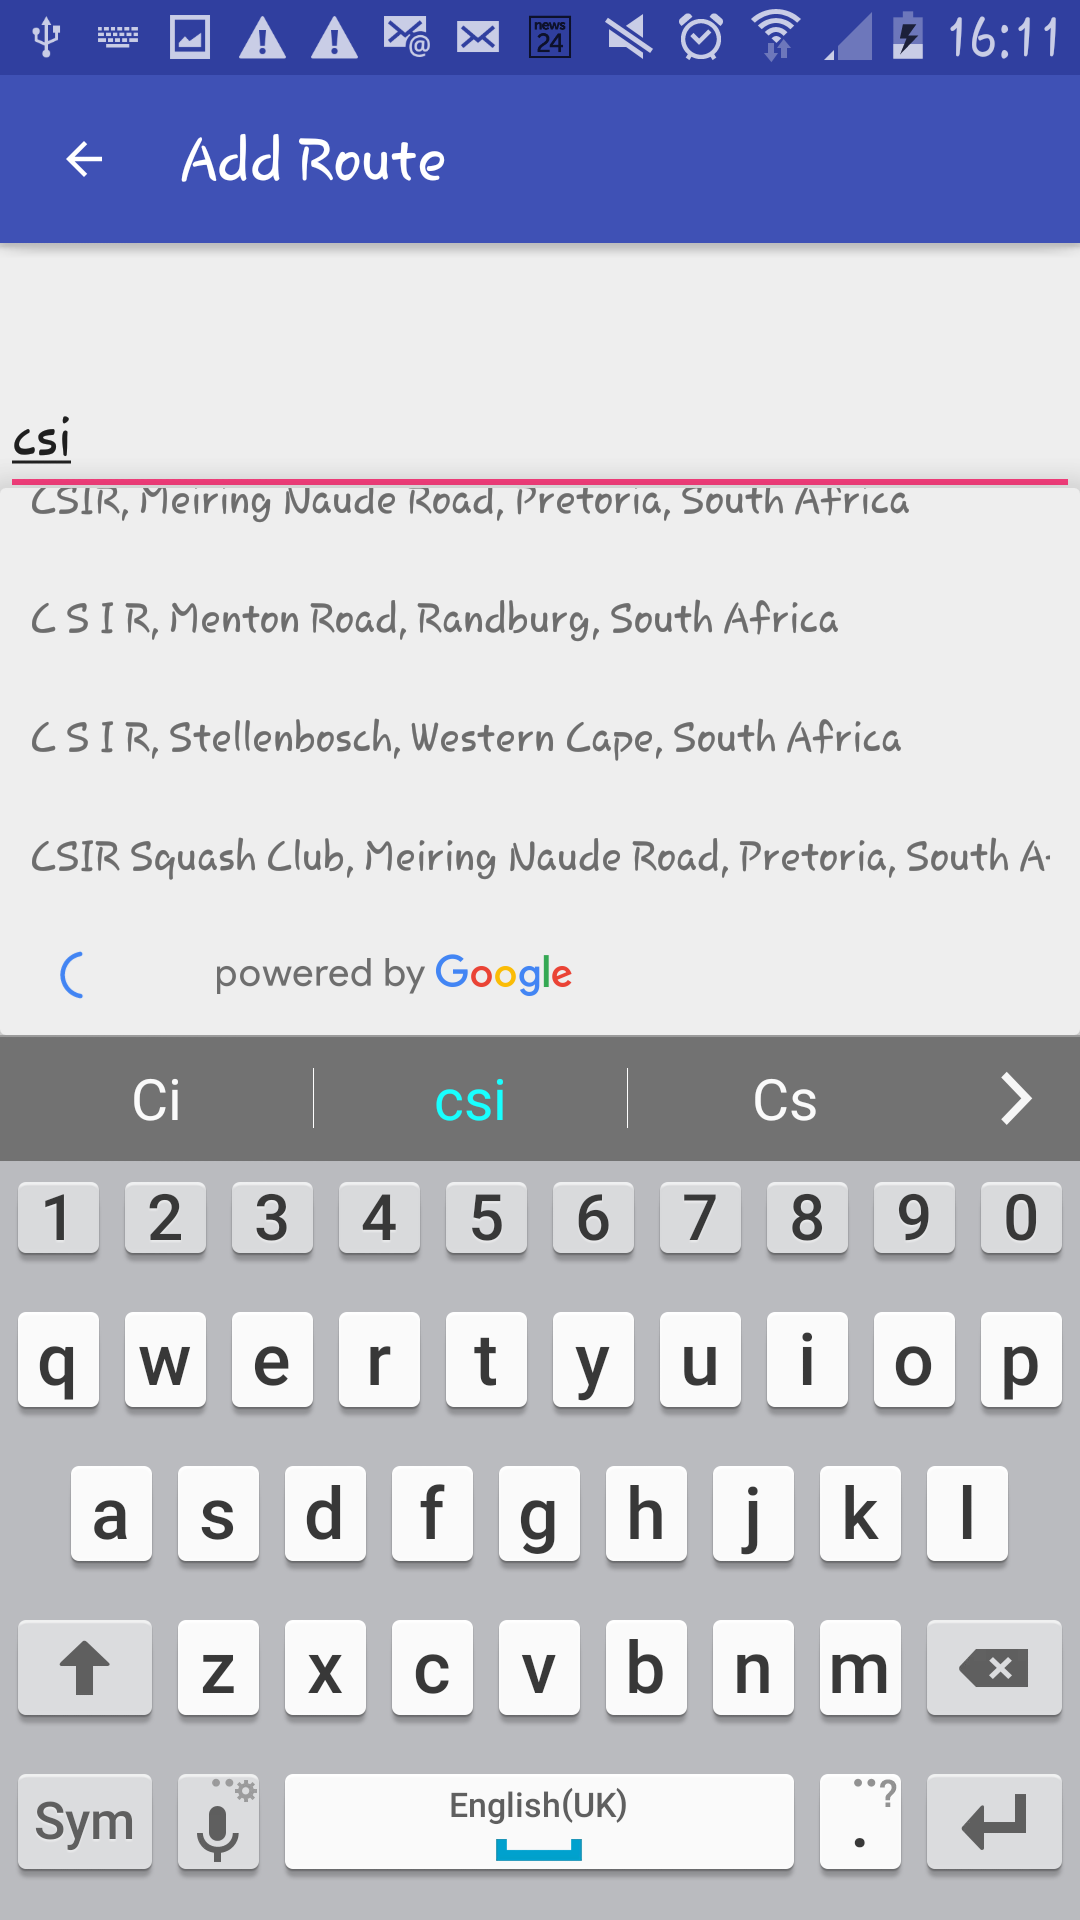
\includegraphics[width=50mm, scale=0.5]{images/AddRoute2.png}
\end{center}
\begin{itemize}
    \item On the application bar which is located at the top of the main screen, click on the plus icon.
    \item The add route screen appears and three input fields will be displayed  where you can enter a start location,an end location and the notification times. Once they have been entered, you then press the find route button and a route will be set up
    \item 
\end{itemize}
\subsubsection{Modifying a Route}
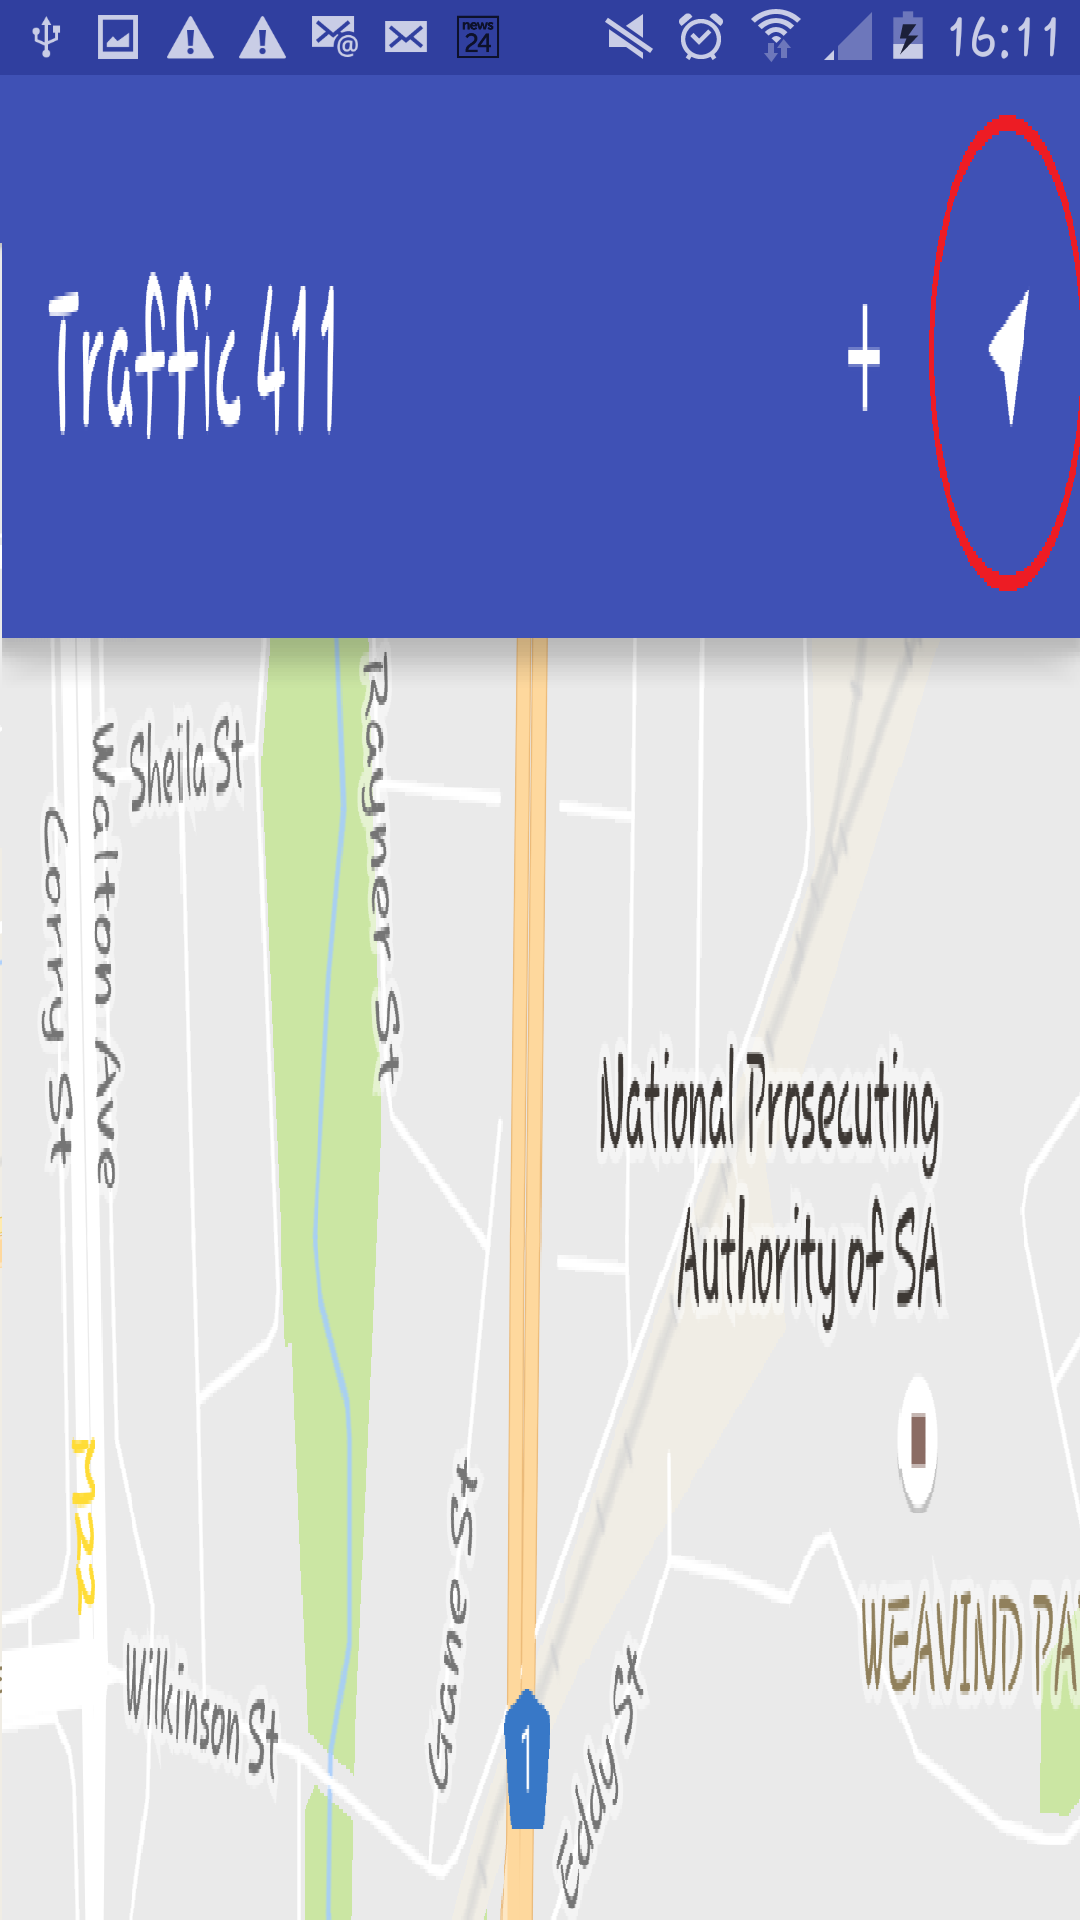
\includegraphics[width=50mm, scale=0.5]{images/MainScreen3.png}
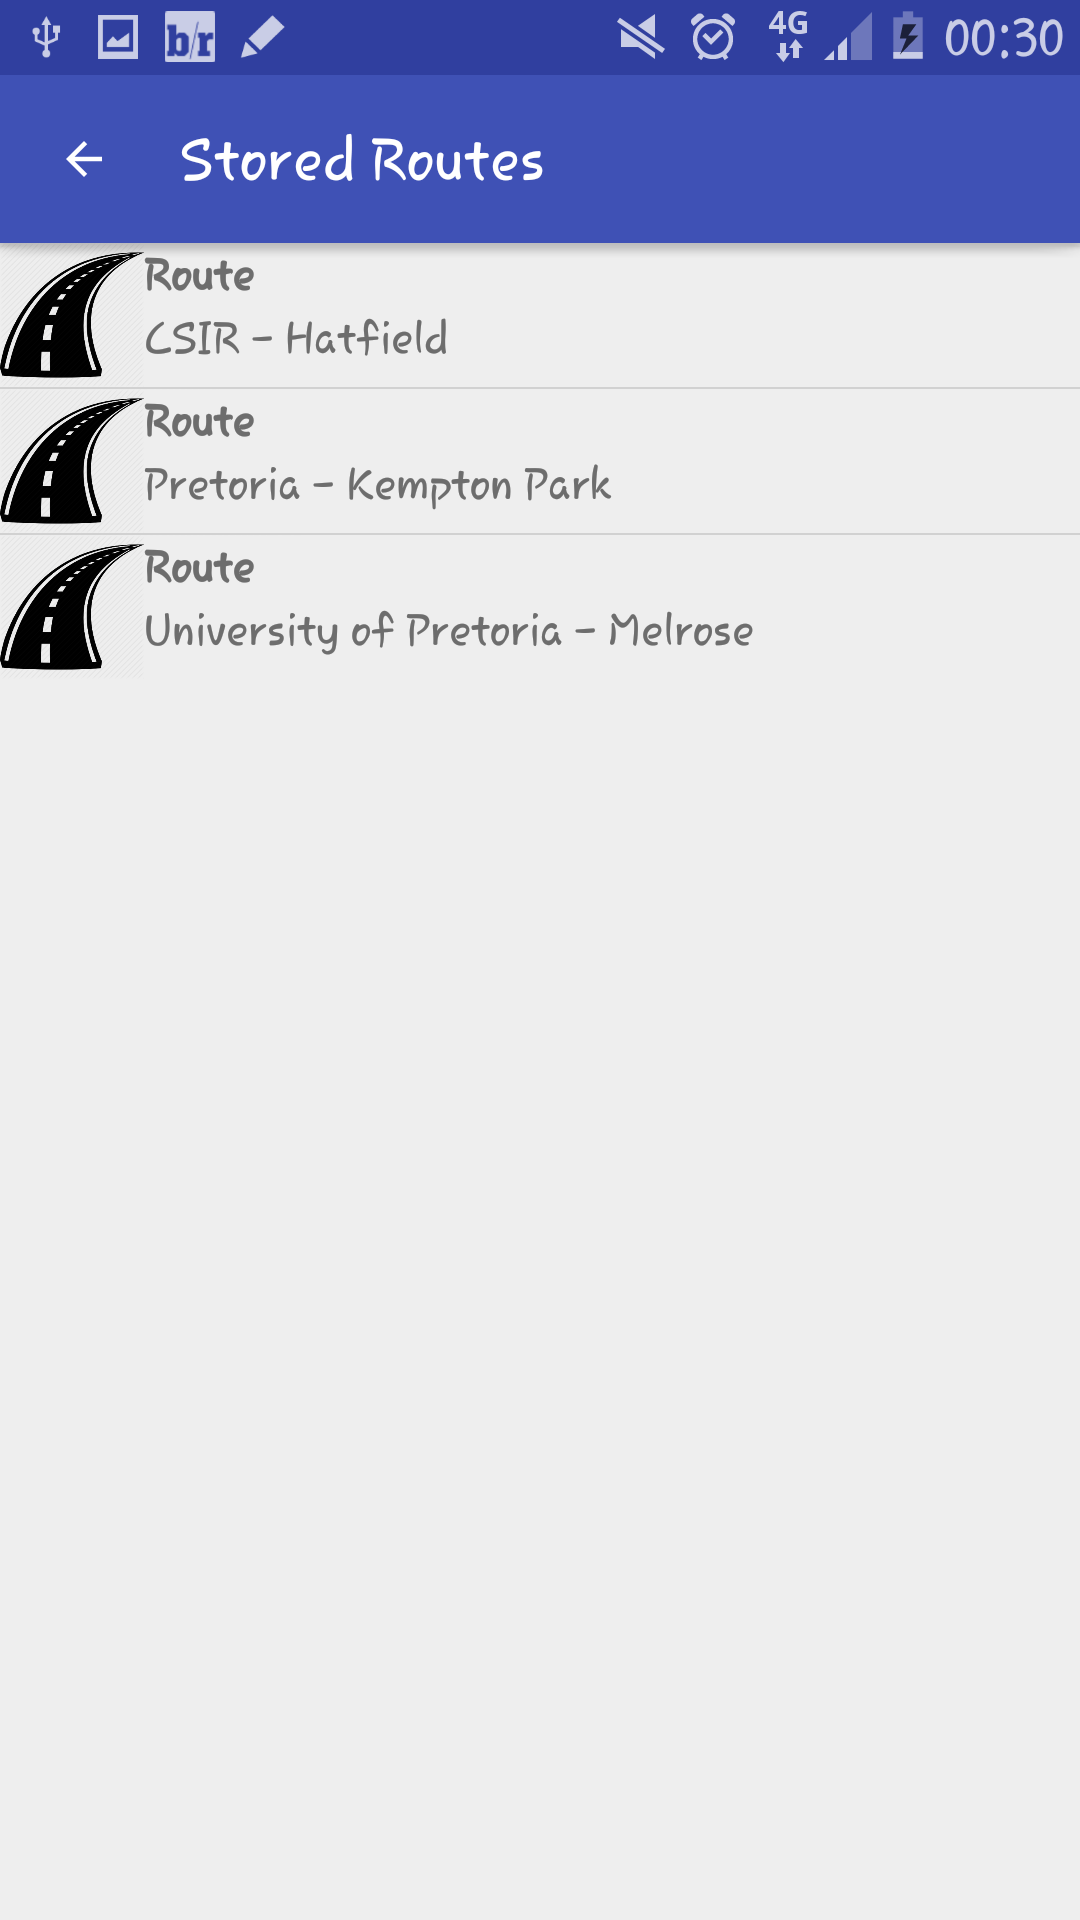
\includegraphics[width=50mm, scale=0.5]{images/StoredRoutes2.png}
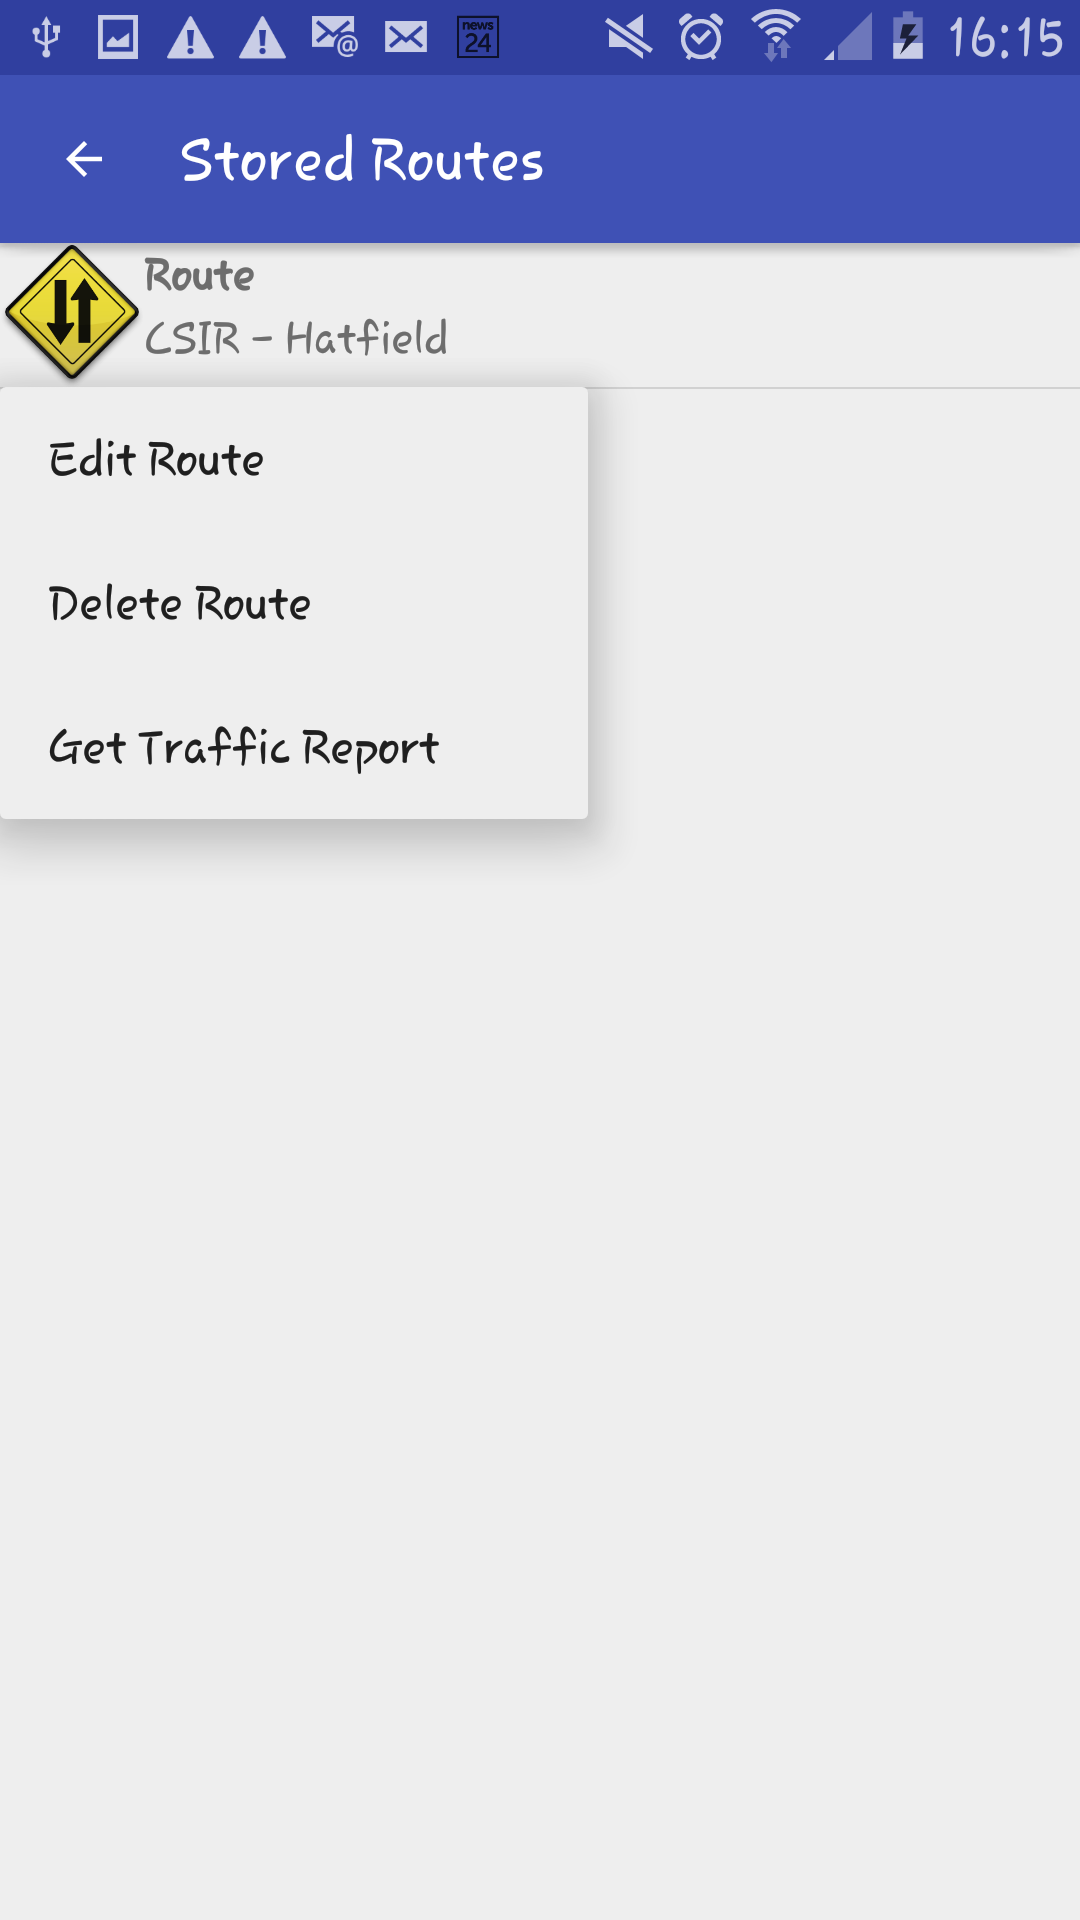
\includegraphics[width=50mm, scale=0.5]{images/Options.png}
\begin{center}
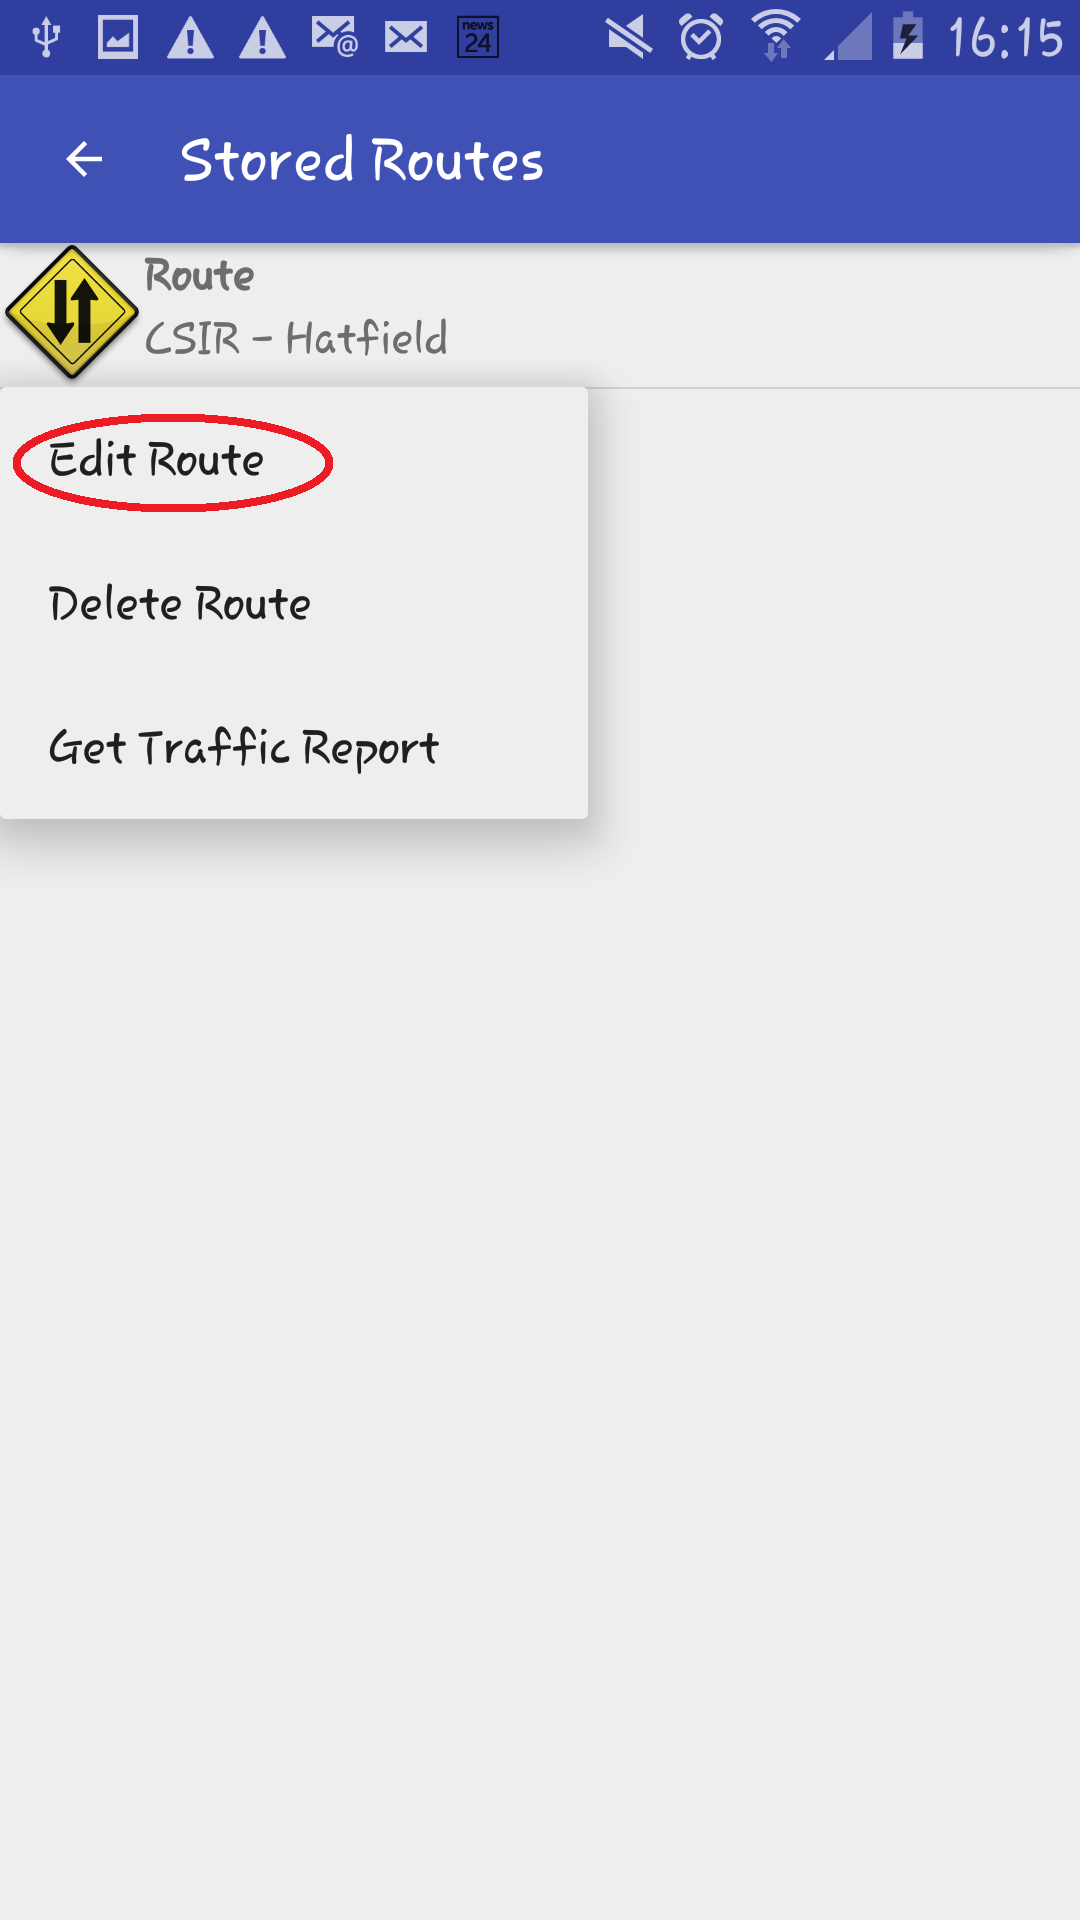
\includegraphics[width=50mm, scale=0.5]{images/EditOption.png}
\end{center}
%Include Image of the actual modify screen
The process of deleting a route is as follows:
\begin{itemize}
    \item First access your stored routes by  clicking on the icon located at the top right corner of the application bar. 
    \item Long click on the route you want to modify, a pop up menu with a list of options will appear.
    \item Click on the Edit Route option.
    \item Once the above step has been executed, two input fields will be displayed  where you can modify either the start location ,end location, the notification times  or all of them. Once they have been entered, you then press the send button and the route will be modified.
\end{itemize}
\subsubsection{Delete a Route}
The process of deleting a route is as follows:
\begin{center}
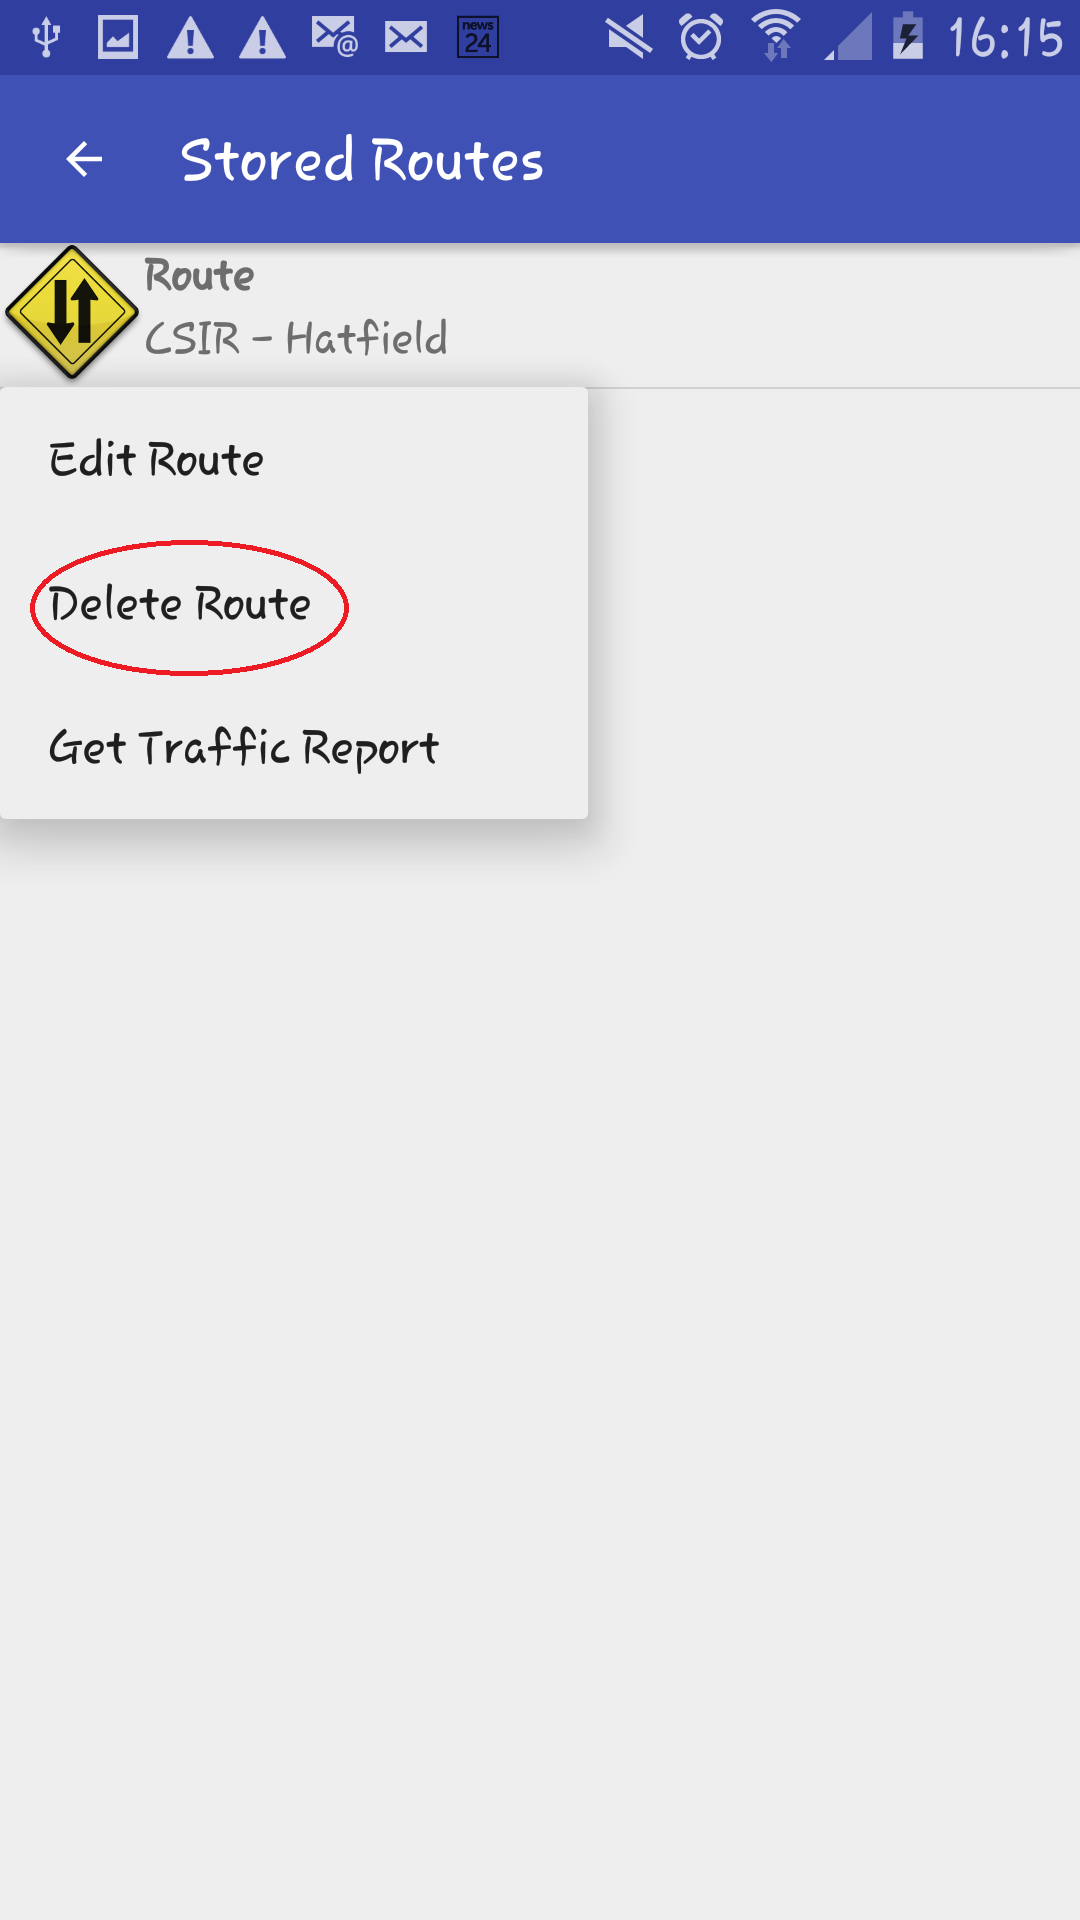
\includegraphics[width=50mm, scale=0.5]{images/DeleteOption.png}
\end{center}
%include screen shots of the delete 
\begin{itemize}
    \item First access your stored routes by  clicking on the icon located at the top right corner of the application bar. 
    \item Long click on the route you want to delete, a pop up menu with a list of options will appear.
    \item Click on the Delete Route option.
\end{itemize}
\subsubsection{Get Traffic Information}
The process of getting the traffic information is as follows:
<<<<<<< HEAD
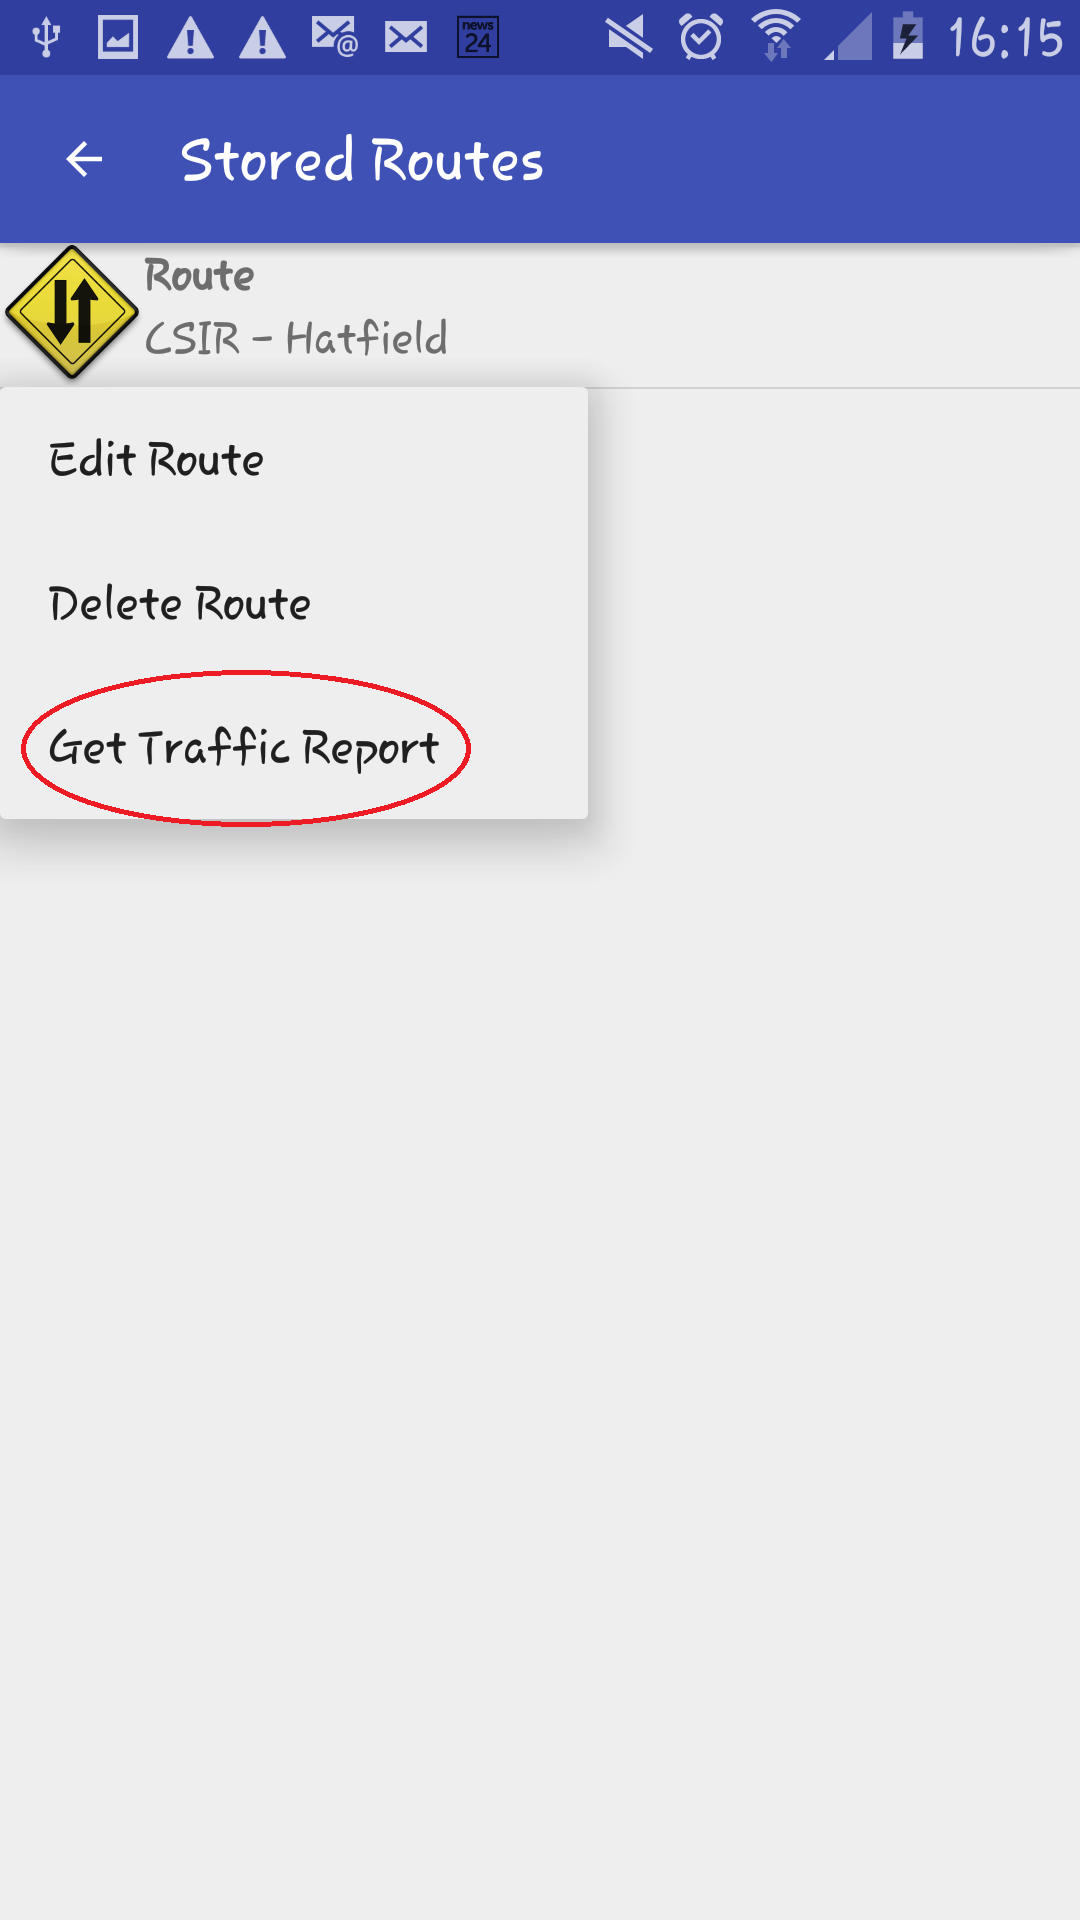
\includegraphics[width=\textwidth]{images/TrafficReportOption.png}
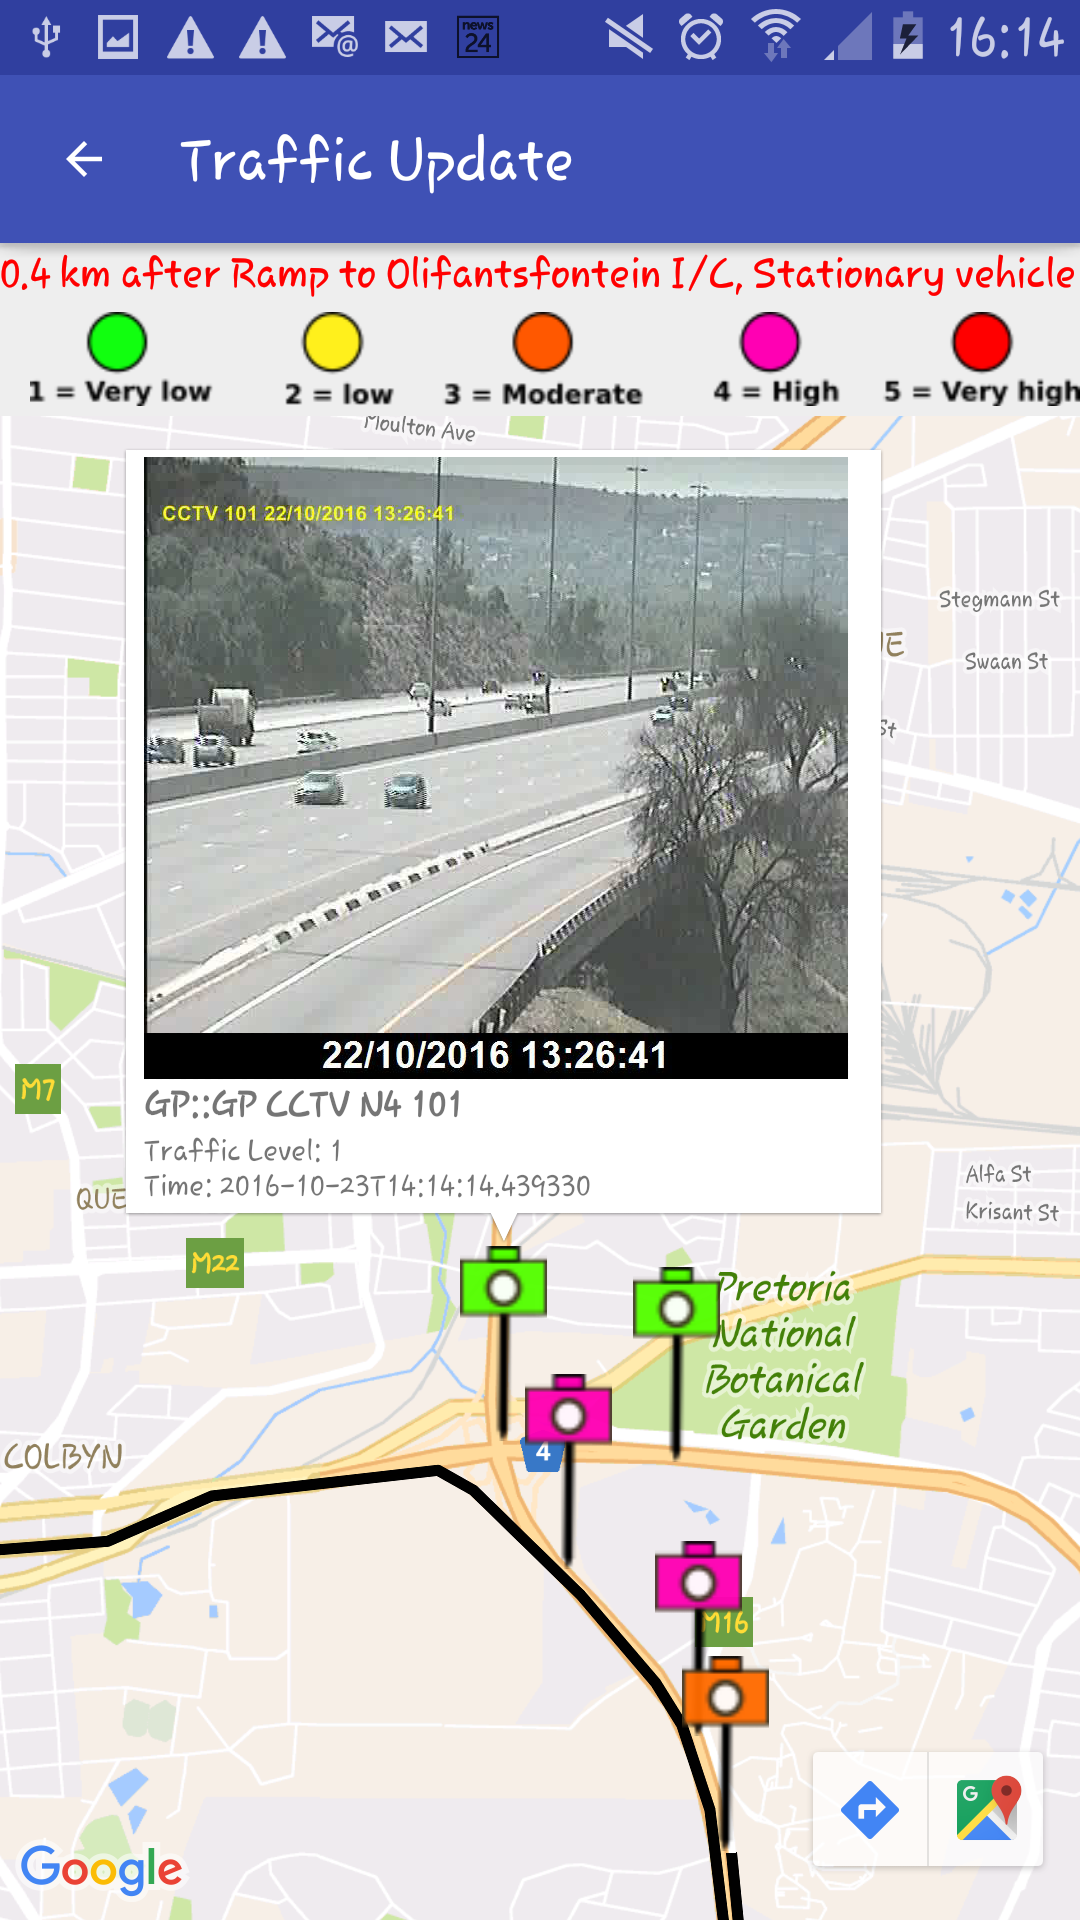
\includegraphics[width=\textwidth]{images/TrafficReport4.png}
=======
\begin{center}
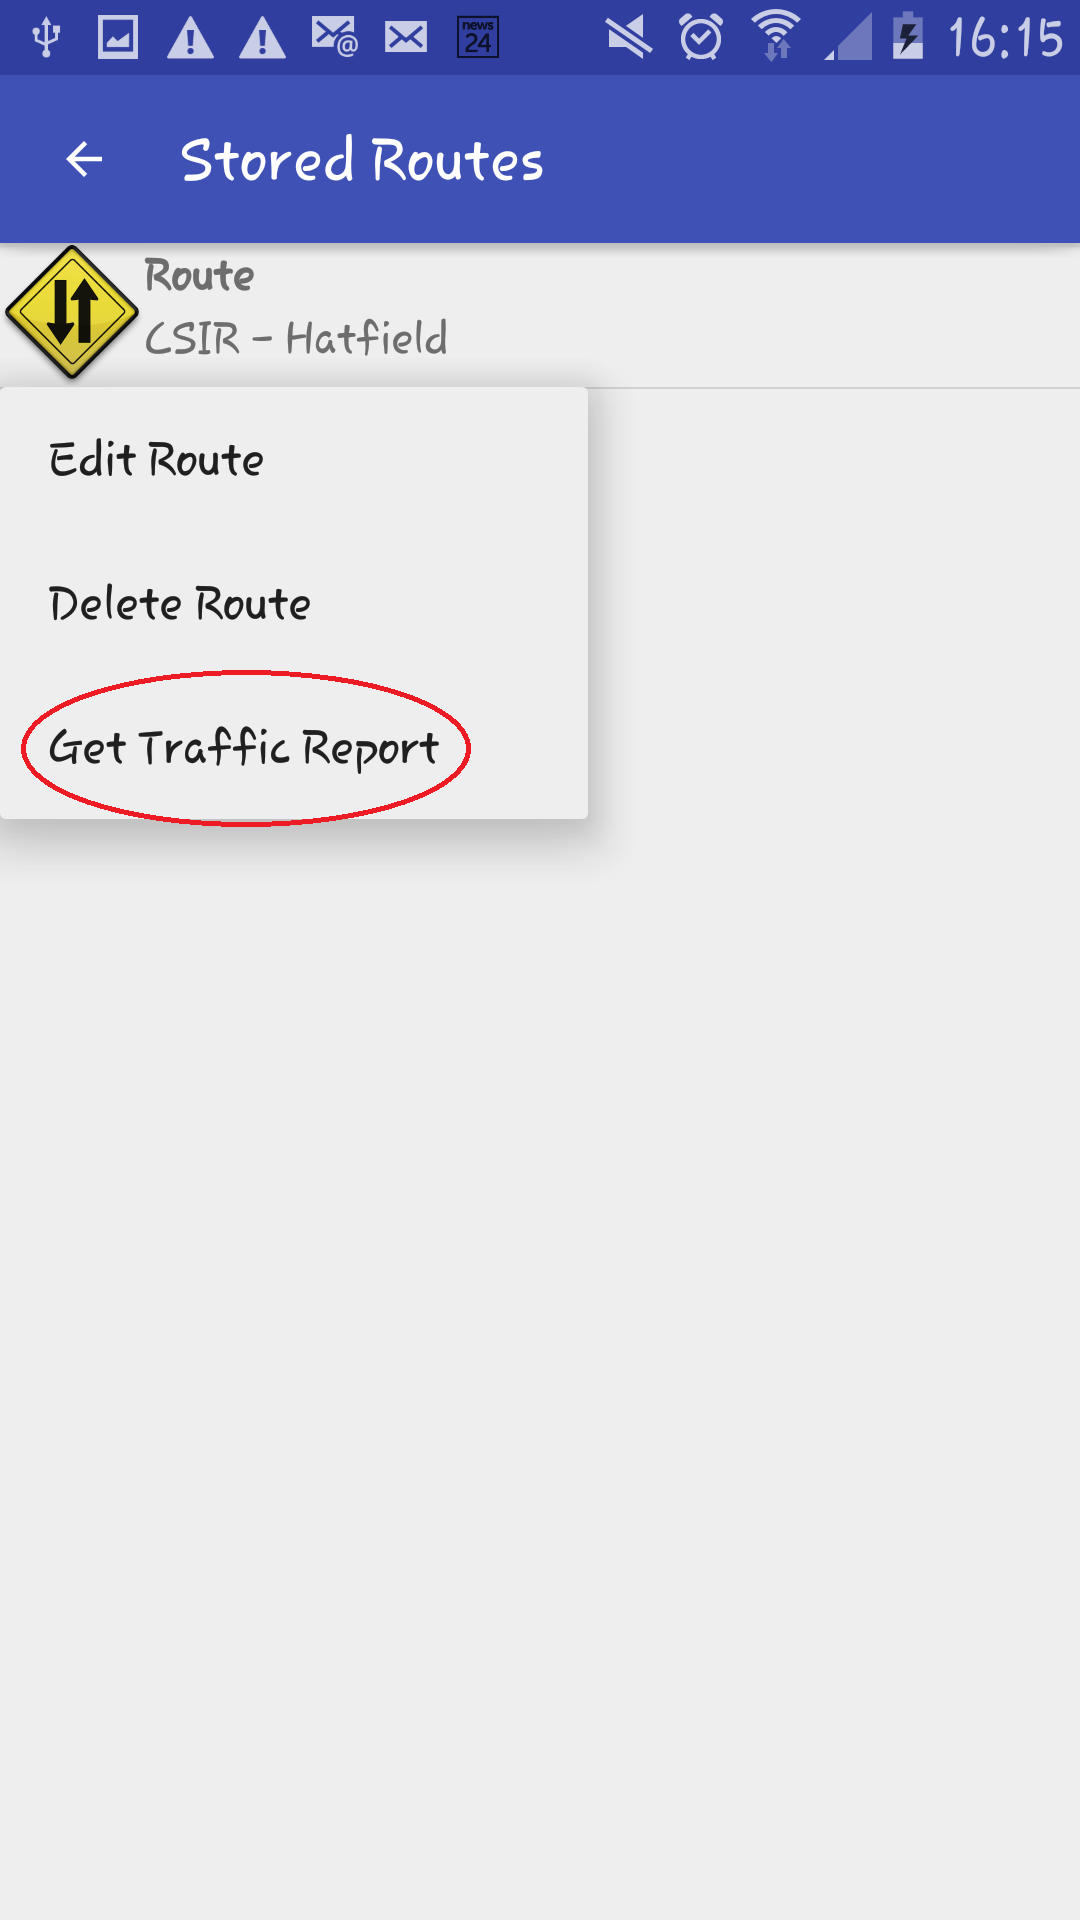
\includegraphics[width=50mm, scale=0.5]{images/TrafficReportOption.png}
\end{center}
\begin{center}
\includegraphics[width=50mm, scale=0.5]{images/TrafficReport.png}
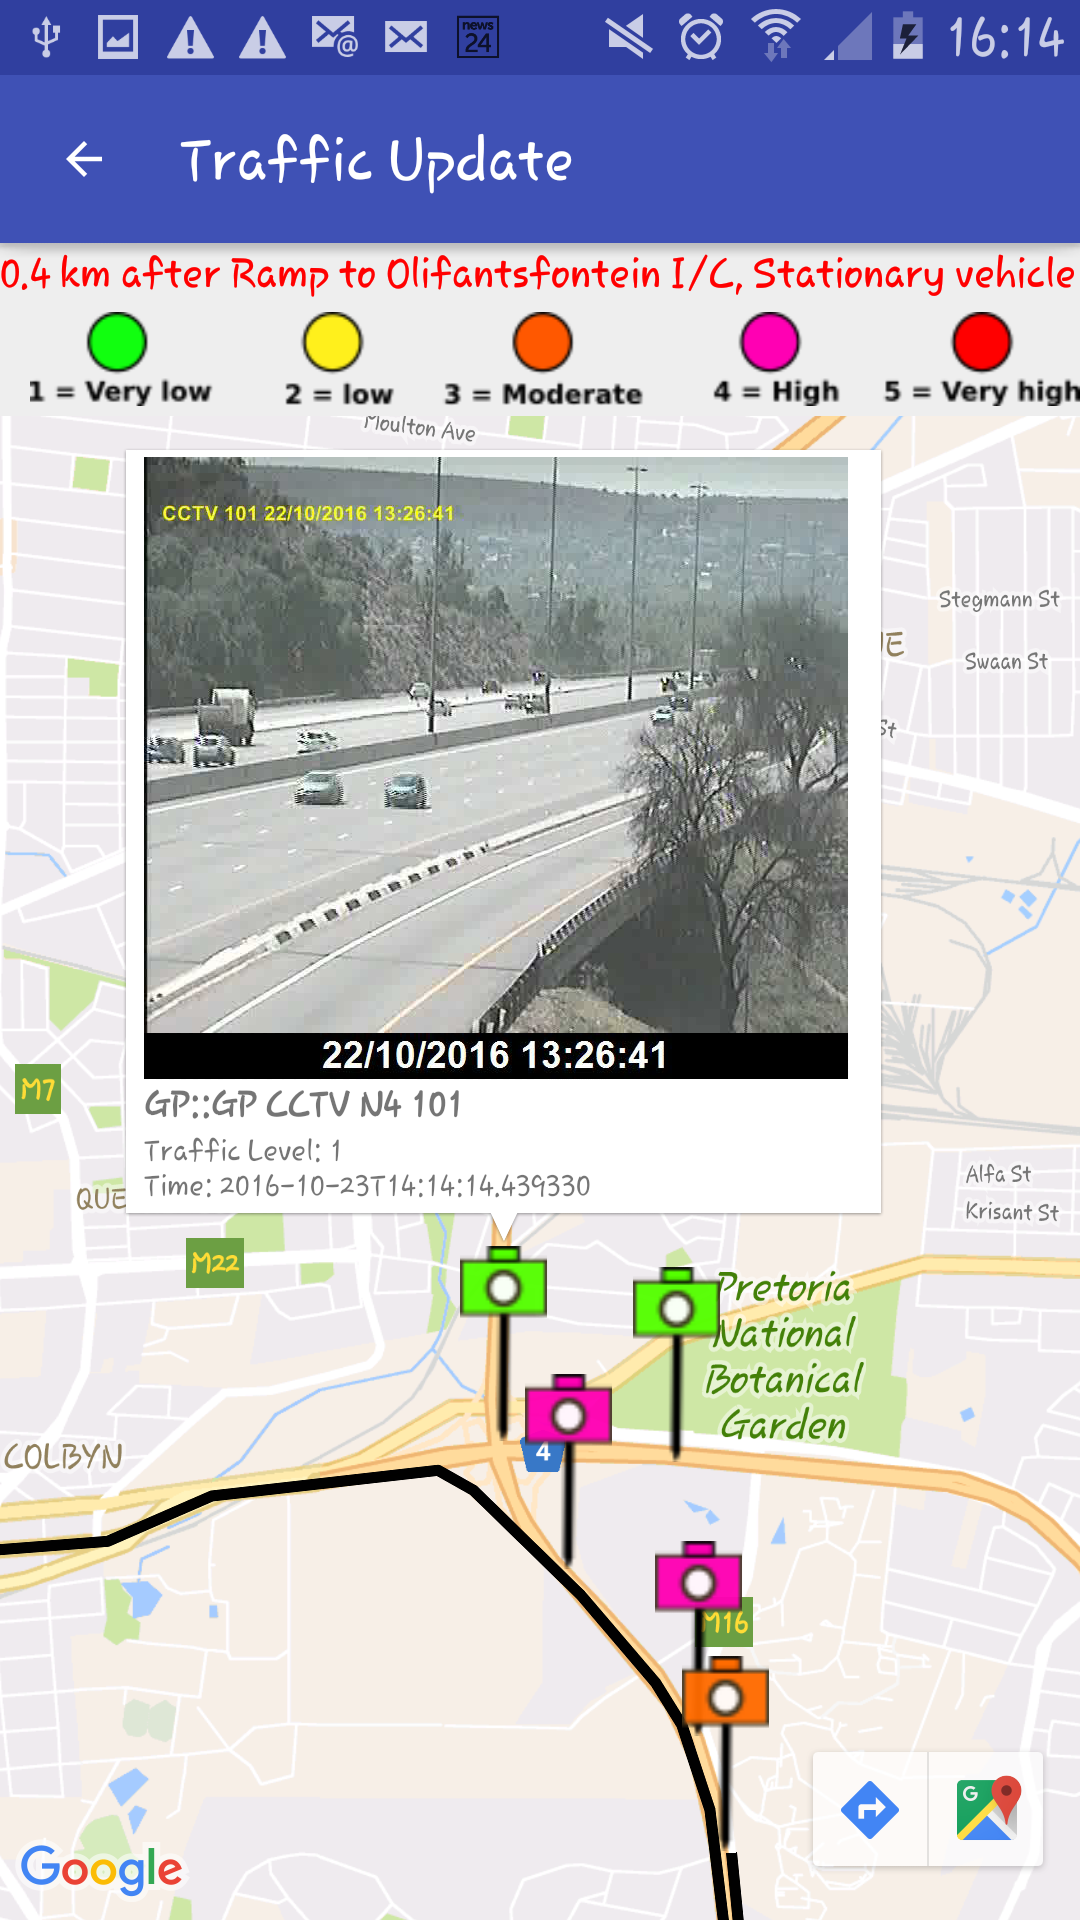
\includegraphics[width=50mm, scale=0.5]{images/TrafficReport4.png}
\end{center}
>>>>>>> 4fb914f7de7a370f4cfd1de83509887d9d6942a3
%Add anything that I might have missed
\begin{itemize}
    \item First access your stored routes by  clicking on the icon located at the top right corner of the application bar. 
    \item Long click on the route for which you require traffic information for., a pop up menu with a list of options will appear.
    \item Click on the Get Traffic Report option.
    \item The traffic update screen will appear, displaying the different traffic level scales at the top , a map showing the different   traffic levels on your route. 
    \item To view the live images of the traffic, click on the camera icons displayed on the map.
\end{itemize}
\end{document}
